\documentclass[12pt,draftcls,onecolumn]{IEEEtran}
\usepackage[utf8]{inputenc}
\usepackage[dvips]{graphicx}
% Title Page
\title{Loss recovery and tail loss performance in Multipath TCP}
\author{KAU}

\begin{document}
\maketitle

\begin{abstract}
\end{abstract}

\section{Introduction}
TCP has two mechanisms for detecting and recovering from packet losses namely Fast Recovery (FR) and Retransmission Timeouts(RTOs). For long flows where there are sufficiently large number of packets 
to be transferred, FR is quicker than RTOs in detecting and recovering packet losses. On the other hand shorter flows which are a majority in the web traffic have to depend on RTOs for packet loss detection 
and recovery incurring more latency. A single packet loss in a short flow may take many RTTs to detect and recover. This scenario is also applicable to the packets at the end of the flow (or tail) in a long 
flow.

TCP Loss Probe (TLP)~\cite{ietftlp} a mechanism that allows flows to detect and recover from tail losses much faster than an RTO, thereby speeding up short transfers. With TLP a packet loss in the middle 
of a packet train as well as at the tail end will now trigger the same fast recovery mechanisms. It assumes other algorithms such as early retransmit~\cite{rfc5827} and FACK threshold based recovery are 
present.

In Multi-path-TCP(MPTCP)~\cite{rfc6824}, a connection can have multiple TCP sub flows using different interfaces on different routes. Packet losses in each sub flow are assumed to be detected and recovered 
in a similar fashion as that of TCP. However, It is not completely clear how the loss recovery happens in the implementation and which sub-flow retransmits the lost packets. If the recovery is handled at the 
meta level, the lost packet may be rescheduled and retransmitted at the available sub flow with lowest RTT. If the recovery is handled at the flow level, the packet may be retransmitted in the same sub-flow. 

Through this set of preliminary experiments, we would like to understand the behavior of MPTCP with and without TLP and ER by monitoring burst completion time, congestion window evolution and timeout 
behavior.
\section{Related Work}\label{relwork}

\section{Scope}\label{scope}

We try to understand the loss recovery and retransmission policies in state of the art MPTCP linux implementation.

\section{Experimental Setup}\label{exsetup}

Planned experiments use CORE emulation platform with a simple topology as depicted in Figure~\ref{fig1}.
Client is connected to two wireless interfaces 3G and WLAN. Server is connected to a wired router.
Characteristics of the connection setup and assumptions about the parameters are provided in table~\ref{tab1}.
Traffic generation is planned with iperf, netperf and d-itg as different runs. 
 
\begin{figure}[!ht]
\begin{center}
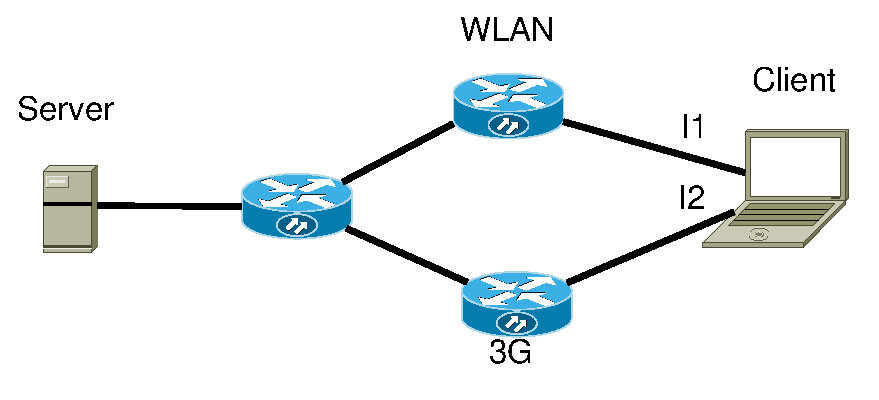
\includegraphics[angle=0, width=0.9\textwidth]{images/fortest.ps}
\caption{Topology used for Emulation}\label{fig1}
\end{center}
\label{prl}
\end{figure}
\begin{center}
\begin{table}
\begin{center}
\begin{tabular}{|c|cccccccccc|}
      \hline
      \multicolumn{1}{c}{} & & \\[\dimexpr-\normalbaselineskip-\arrayrulewidth]
      \textbf{Burst Size} & \multicolumn{10}{c|}{160 Packets} \\
      \hline
      \textbf{Separation Time} & \multicolumn{10}{c|}{2s} \\
      \hline

      \textbf{Run Length} & \multicolumn{10}{c|}{10min}\\
      \hline 	
      \textbf{RTT} & \multicolumn{5}{c|}{200ms(3G)} & \multicolumn{5}{c|}{20ms(WLAN)} \\
      \hline 	
      \textbf{Bandwidth} & \multicolumn{5}{c|}{7Mbps(3G)} & \multicolumn{5}{c|}{54Mbps(WLAN)} \\
      \hline
      \textbf{Loss} & \multicolumn{5}{c|}{0(3G)} & \multicolumn{5}{c|}{2\%(WLAN)} \\
      \hline
      \textbf{Loss Model} & \multicolumn{10}{c|}{Random}\\
      \hline
\end{tabular}
\caption{Connection parameters}\label{tab1}
\end{center}
\end{table}
\end{center}


\subsection{Testing with Deterministic loss patterns}
In order to understand the retransmission behavior of the Linux MPTCP implementation and to reproduce the observed retransmissions, we use a deterministic drop pattern.
Losses generated by using associating netem with corresponding interfaces and dropping the packets(Cite KAU paper). 
 


\section{Observations and Discussion}\label{disc}
Preliminary experiments on CORE emulator with the setup mentioned in section\ref{exsetup} showed several cases where the behavior on losses differ.


\section{Tail loss scenarios}
We tried to understand the behavior of MPTCP retransmissions at different flow levels in the following tail loss scenarios~\ref{ret3}.
MPTCP is sensitive to path asymmetry in general due to the default scheduler being shortest RTT based scheduler. Wireshark and tcptrace
analysis provides information on the TCP retransmissions at the meta level. mptcptrace provides information on flow sequence split at 
subflow level. Subflow level retransmissions are difficult to test from the output of mptcptrace analysis. Further deep packet inspection
is required to understand the losses at the subflow level.

\begin{table}[]
\centering
\caption{Tail loss scenarios with tcp.early.retrans = 3 default}
\label{ret3}
\begin{tabular}{|l|l|l|l|l|}
\hline
 testcase   & Asymmetry   & Metalevel          & Subflowlevel       &  \\\hline
Tail drop 1 & 20ms - 30ms & rexmt in same path & rexmt in same path &  \\\hline
Tail drop 2 & 30ms - 20ms & rexmt in same path & TBC                &  \\\hline
Tail drop 3 & 20ms - 20ms & rexmt in same path & TBC                &  \\ \hline
\end{tabular}
\end{table}





\begin{table}[]
\centering
\caption{Tail loss scenarios with tcp.early.retrans = 0 ER disabled}
\label{ret3}
\begin{tabular}{|l|l|l|l|l|}
\hline
 testcase   & Asymmetry   & Metalevel          & Subflowlevel       &  \\\hline
Tail drop 1 & 20ms - 30ms & rexmt in same path & rexmt in same path &  \\\hline
Tail drop 2 & 30ms - 20ms & rexmt in same path & TBC                &  \\\hline
Tail drop 3 & 20ms - 20ms & rexmt in same path & TBC                & \\ \hline
Tail drop 4 & 20ms - 120ms &  			&		&  \\ \hline
Tail drop 5 & 120ms - 20ms &  			& 		& \\ \hline 
\end{tabular}
\end{table}


\begin{table}[]
\centering
\caption{Tail loss scenarios with tcp.early.retrans = 4 TLP disabled}
\label{ret3}
\begin{tabular}{|l|l|l|l|l|}
\hline
 testcase   & Asymmetry   & Metalevel          & Subflowlevel       &  \\\hline
Tail drop 1 & 20ms - 30ms & rexmt in same path & rexmt in same path &  \\\hline
Tail drop 2 & 30ms - 20ms & rexmt in same path & TBC                &  \\\hline
Tail drop 3 & 20ms - 20ms & rexmt in same path & TBC                & \\ \hline
\end{tabular}
\end{table}

The linux sysctl setting tcp\_early\_retrans is 3 by default. This option enables both Early retransmit and TLP. 
Further testcases should be considered with options 0 and 4. 

\section{Improvements to TLP}
The goal of Tail Loss Probe(TLP) is to reduce tail latency of short flows. It achieves this by converting retransmission timeouts (RTOs) occuring due to tail losses (losses at end of transactions) into fast recovery. TLP transmits one packet in two round-trips when a connection is in Open state and isn't receiving any ACKs. The transmitted packet, aka loss probe, can be either new or a retransmission. When there is tail loss, the ACK from a loss probe triggers FACK/early-retransmit based fast recovery, thus avoiding a costly retransmission timeout.

Current implementation of TLP is at the TCP flow level. In the event of RTO timeout the MPTCP retransmission happens with a reinjection in to scheduler along with sending lost packet on the same path. But in the Event of Probe timeout, the lost packet is being sent on the same path without injecting in to scheduler.  Modifications should reinject the lost packet in to the mptcp scheduler in the event of PTO.

\subsection{Example scenario where MPTCP TLP could incur more latency}

Use a traffic pattern where there is new burst to send before the RTO after a tail loss triggering TLP on a flow.


\section{Proposed changes and expected implications}


\subsection{Implementation Plan}

Things to do:



When PTO fires: in code trigger call on PTO in tcp level
It calls ${tcp\_push\_one()}$ in tcp-output.c and then ${mptcp\_write\_xmit()}$.
As it is reinjection (due to only one case currently in MPTCP), that packet will have path mask
to put it on the same subflow. Here we need to add a case for reinjection due to PTO that should
send the packet to $reinject\_queue$ of ${mptcp\_cb}$ as well.


Main flow packet queue and subflow packet queue: ${meta\_sk}$ refers to the
main mptcp flow.

Loss probe timer used in Linux: ${ICSK\_TIME\_LOSS\_PROBE}$.

\section{Evaluation of proposal}

Initial testing with customized program to send bursts of packets with fixed burst seperation. Adjust the burst seperation to get the desired scenario.





\bibliographystyle{IEEEtran}
\bibliography{mptcp-retrans}
\end{document} 
